\documentclass[12pt, a4papre]{article}
\usepackage[catalan]{babel}
\usepackage[unicode]{hyperref}
\usepackage[dvipsnames]{xcolor}
\usepackage{amsmath}
\usepackage{amssymb}
\usepackage{amsthm}
\usepackage{xifthen}
\usepackage{siunitx}
\usepackage{xcolor}
\usepackage{float}
\usepackage{listings}
\usepackage{setspace}
\usepackage{graphicx}
\usepackage{tikz,lipsum,lmodern}
\usepackage[most]{tcolorbox}
\usepackage{multicol}
\usepackage{fancyvrb}
\usepackage{circuitikz}
\usepackage{indentfirst}
\usepackage{verbatimbox}
\usepackage{verbatim}
\usepackage[utf8]{inputenc}
\definecolor{mygreen}{RGB}{28,172,0} % color values Red, Green, Blue
\definecolor{mylilas}{RGB}{170,55,241}
\graphicspath{ {./Images/} }

\newcommand{\norm}[1]{\lvert #1 \rvert}

\hypersetup{
    colorlinks = true,
    linkcolor = blue
}
\newtheorem*{theorem*}{Theorem}
\newtheorem*{lemma}{Prop}

\usepackage{xcolor}
\usepackage{listings}
\lstloadlanguages{Python}
\lstset{
  language=Python,
  basicstyle=\scriptsize\sffamily,
  numberstyle=\color{gray},
  stringstyle=\color[HTML]{933797},
  commentstyle=\color[HTML]{228B22}\sffamily,
  emph={[2]from,import,pass,return}, emphstyle={[2]\color[HTML]{DD52F0}},
  emph={[3]range}, emphstyle={[3]\color[HTML]{D17032}},
  emph={[4]for,in,def}, emphstyle={[4]\color{blue}},
  showstringspaces=false,
  breaklines=true,
  prebreak=\mbox{{\color{gray}\tiny$\searrow$}},
  numbers=left,
  xleftmargin=15pt
}

\author{Daniel Vilardell}
\title{Exercici Difusió Calor ALN}
\date{Març 2021}

\begin{document}
	\maketitle
	
	\textbf{a)} Calculem primer el cost de l'eliminació Gaussiana en banda, i després el de la substitució enrera en banda. L'eliminació gaussiana te tres fors, un de mida n i dos de mida min(n - i, s) on i es la variable d'iteració del primer. El mes interior té una operació i el intermig en té 2. Sigui m = min(n, i + s) aleshores
	\[
		\sum_{i = 1}^n\sum_{j = i + 1}^{m}(2+ \sum_{j = i + 1}^{m}1) \approx \sum_{i = 1}^n\sum_{j = i + 1}^{m}\sum_{j = i + 1}^{m}1 = \sum_{i = 1}^{n - s}\sum_{j =  1}^{s}\sum_{j =  1}^{s}1 + \sum_{i = n - s + 1}^{n}\sum_{j =  i + 1}^{n}\sum_{j =  i + 1}^{n}1
	\]
	
	Observem que el segon sumatori es el mateix que el que vam trobar al buscar el nombre d'operacions del metode de gauss pero en aquest cas en una matriu de mida sxs, per tant el ordre del nombre d'operacions es $\Theta (s^3)$.
	\[
		\#operacions \approx (n - s)s^2 + \Theta (s^3)
	\]
	
	Si considerem que $n >> s$ aleshores 
	\[
		\#operacions = \Theta (ns^2)
	\]
	
	El cost de aplicar a substitució enrere, si considerem altre cop $n >> s$ es el següent
	\[
		\#operacions = \sum_{i = 1}^n\sum_{j = i + 1}^{m}1 = \Theta (ns)
	\]
	
	Cal apuntar però que el simple fet de crear la matriu ja es del ordre de $\Theta (n^2)$ i si, tal com hem considerat, $n >> s \implies n >> s^2$, aleshores el nombre d'operacions total el domina el fet de crear la matriu mes que resoldre el sistema.
	\[
		\#operacions_{tot} =  \Theta (n^2) + \Theta (ns^2) +  \Theta (ns) =  \Theta (n^2)
	\]
	
	Si nomes ens guardessim la banda de la matriu i no ens guardessim els 0 aleshores això no seria problema, tot i que al codi de difusió de calor no es fa així.
	
	\textbf{b)}
	
	\lstinputlisting[language=Python, frame=single]{codis/codi1.py}
	
	A dins del main, per a comprobar que la solució era correcta hem introduit el següent codi.
	
	\lstinputlisting[language=Python, frame=single]{codis/codi2.py}
	
	\newpage
	\textbf{c)}
	En primer lloc hem afegit un for que ens repeteix el codi 10 cops, i cada cop recopilavem les dades, aquí podem veure un resum de 10 iteracions del algoritme, cadascuna amb un refinament diferent. Totes les dades son aplicant l'algoritme de eliminació Gaussiana en banda.
	\begin{multicols}{2}
	{\scriptsize \VerbatimInput{./codis/informacio_1.txt}}
	\end{multicols}
	
	A partir d'aquestes dades hem graficat el logaritme del temps de calcul en funció del logaritme de la dimensió del sistema i el logaritme del nombre de coeficients no nuls en funció del logaritme de la dimensió. 
	
	En la primera i segona grafica podem concloure que el creixement es aproximadament lineal (amb excepcio dels refinaments petits que te un pendent inferior). Tot i això podem veure que el pendent en la funció de Gauss sense banda es de aproximadament $6\cdot 10^{-3}$ mentres que en el Gauss amb banda el pendent es de aproximadament $4\cdot 10^{-4}$, cosa que mostra la gran millora respecte al altre metode.
	
	\begin{figure}[H]
		\begin{center}
		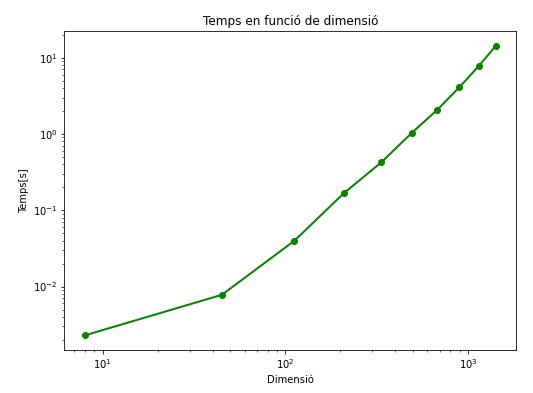
\includegraphics[width=110mm]{t_dim_nob.png}
		\caption{Gauss sense banda}
		\end{center}
	\end{figure}
	
	\begin{figure}[H]
		\begin{center}
		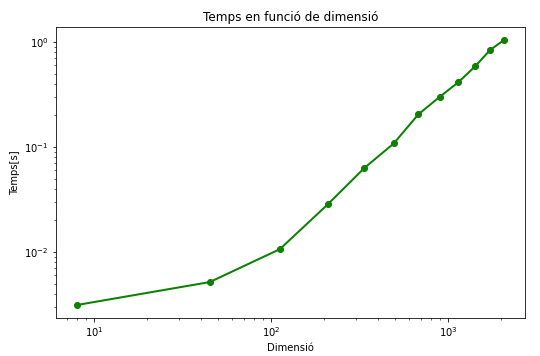
\includegraphics[width=110mm]{t_dim_b.png}
		\caption{Gauss amb banda}
		\end{center}
	\end{figure}
	
	Podem veure per altra banda que el nombre de coeficients no nuls abans de cridar la funció d'eliminació Gaussiana i despres varia bastant, arribant a tenir una proporcio amb el refinament 14 de $\frac{2\cdot 10^5}{1.5\cdot 10^4} \approx 15$. Si calculem el pendent veiem que la primera grafica te pendent de 3 mentres que la segona te un pendent de 100. 
	
	Cal apuntar que la funció np.count\_nonzero conta el nombre d'elements no nuls, i durant el metode de Gauss hi poden haver errors de precisió. Cal per tant contar tots els coeficients que son majors a un epsilon.
	
	\begin{figure}[H]
		\begin{center}
		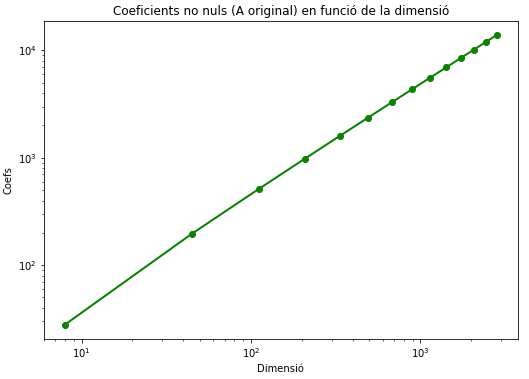
\includegraphics[width=110mm]{coef_dim_or.png}
		\caption{Coeficients no nuls en la matriu original}
		\end{center}
	\end{figure}
	
	\begin{figure}[H]
		\begin{center}
		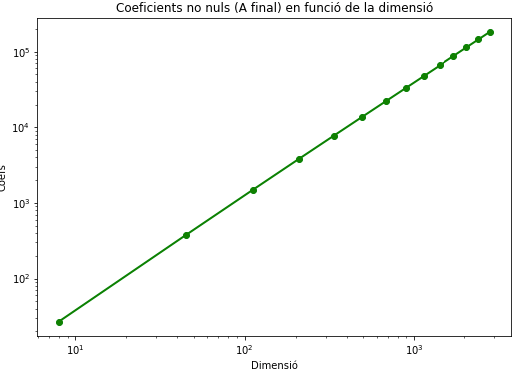
\includegraphics[width=110mm]{coef_dim_fin.png}
		\caption{Coeficients no nuls en la matriu final}
		\end{center}
	\end{figure}
	
	
\end{document}
